\documentclass[11pt]{beamer}
\usetheme{Warsaw}
\usepackage[utf8]{inputenc}
\usepackage{amsmath}
\usepackage{amsfonts}
\usepackage{amssymb}
\usepackage{color}

\usepackage{graphicx}
\usepackage{caption}
\usepackage{subcaption}


\author{Arindam Basu \\ Ion Accelerator Developement Division\\ BARC}
\title{Folded Tandem Ion Accelerator(FOTIA)\\ Overview Operational and Safety Aspects}
%\setbeamercovered{transparent} 
%\setbeamertemplate{navigation symbols}{} 
%\logo{} 
%institute{BARC} 
%\date{} 
%\subject{} 
\begin{document}

\begin{frame}
\titlepage
\end{frame}

%\begin{frame}
%\tableofcontents
%\end{frame}


\begin{frame}{Plan of the talk}

\begin{itemize}
\item Introduction of the FOTIA facility.
\item Types of experiments carried out in FOTIA facility.
\item Safety aspects of FOTIA facility.
\item Conclusions



\end{itemize}

\end{frame}





\begin{frame}{Folded Tandem Ion Accelerator(FOTIA)}

\begin{itemize}
\item \textbf{FOTIA} is a DC electrostatic accelerator.
\item \textbf{FOTIA} is an upgraded version of old Van de Graaf accelerator.
\item \textbf{FOTIA} can deliver variety of positive ion beams for experimentation into various areas of science and technology. It is extensively used by BARC and non BARC users.
\item \textbf{FOTIA} is running very reliably for last ten years and contributed to various programs of DAE.
 
\end{itemize}

\end{frame}


\begin{frame}{FOTIA Specifications}

  \begin{itemize}
   
    \item \textbf{Max Voltage} 6 Mv.
    \item \textbf{Voltage Stability} $\underline{+} 2 kV $.
    \item \textbf{Ions} Positively charged ions with $\dfrac{mE}{q^2}   \leqslant 42$.
    \item \textbf{Max Energy} 1 to 5 Mev for Proton , for heavy ions (n+1)V where n is the charge state and V is the terminal voltage.
    \item \textbf{Max Current} 
    \begin{enumerate}
     \item Proton : 500 nA
     \item Heavy ions( Li , $C^{3+,4+}$ , O , F ): tens of particle nano Amp.
    \end{enumerate}
      
   \end{itemize}

\end{frame}

% new Slide
\begin{frame}{Schematic Diagram of FOTIA}
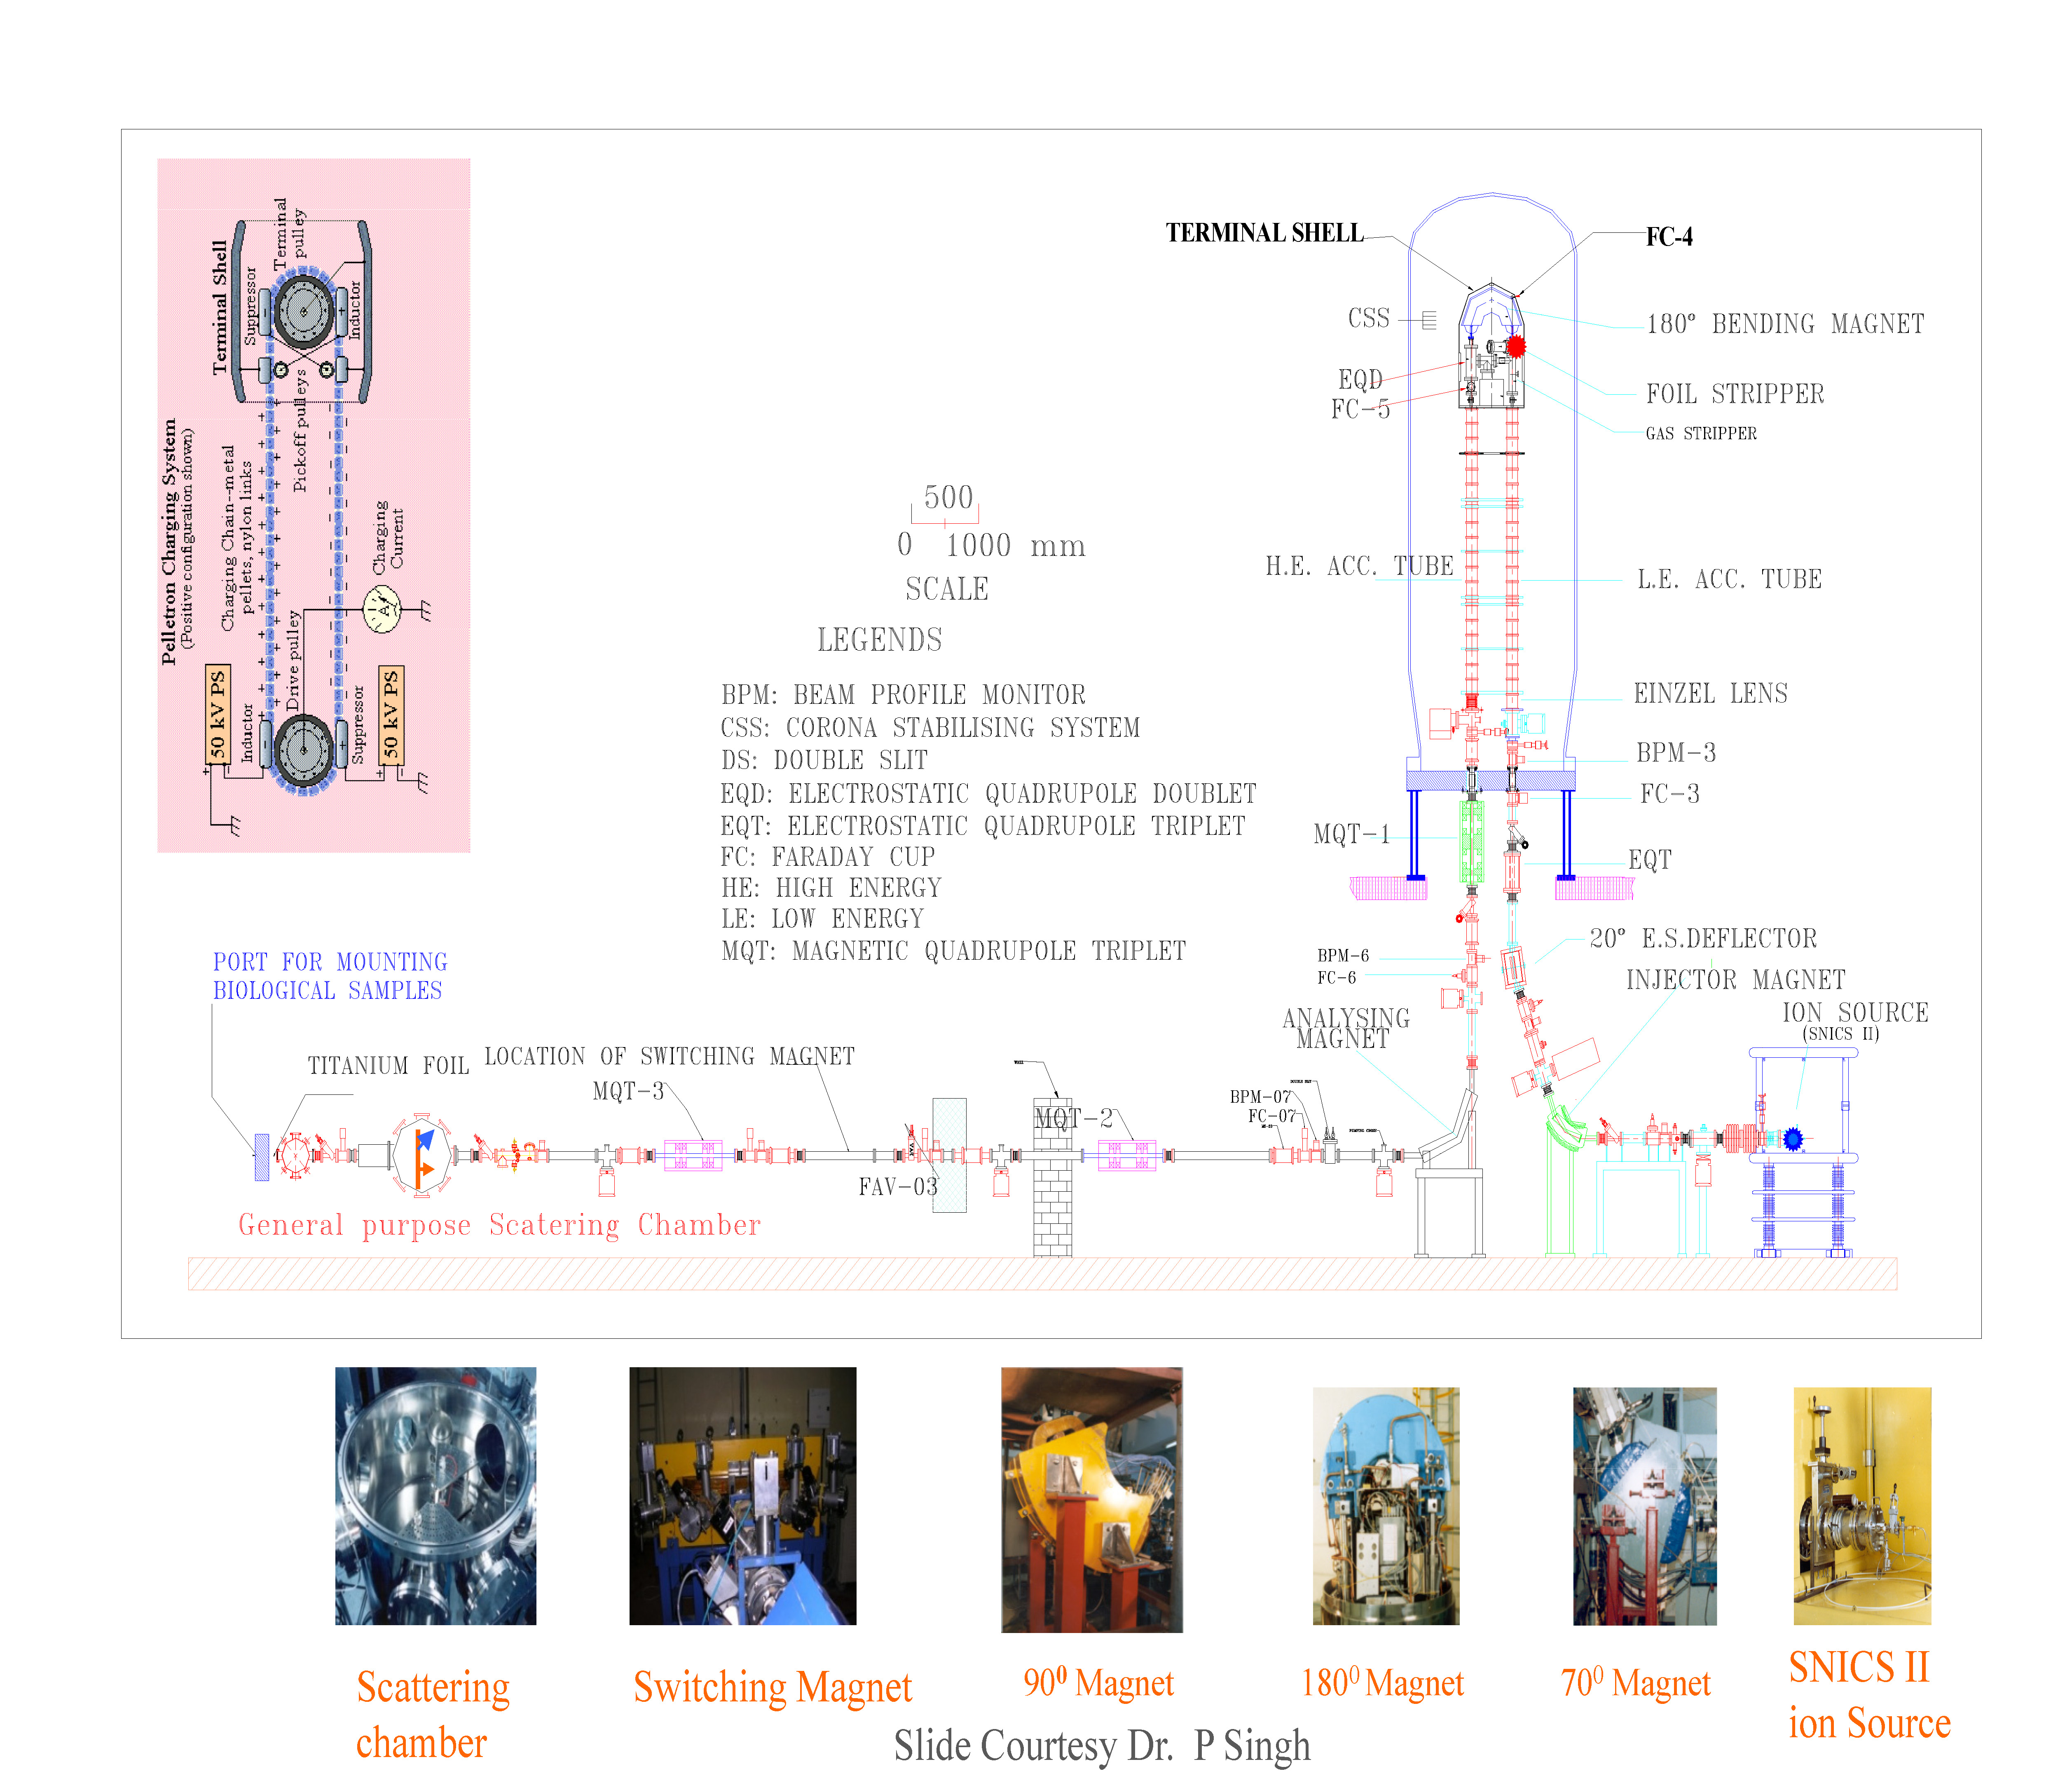
\includegraphics[width=\linewidth]{FOTIA_Page_05.jpg}
\end{frame}


% new Slide
\begin{frame}{FOTIA Subsystems}

  \begin{itemize}
   
    \item Ion Source.
    \item Bending and Focusing devices- electrostatic and magnetic.
    \item High voltage and high current power supplies.
    \item High Voltage generation system.
    \item $SF_{6}$ gas handling system.
    \item Vacuum system.
    \item Control and instrumentation system.
   \end{itemize}

\end{frame}

% new Slide
\begin{frame}{FOTIA Subsystems-Ion Source}

   \begin{center}
    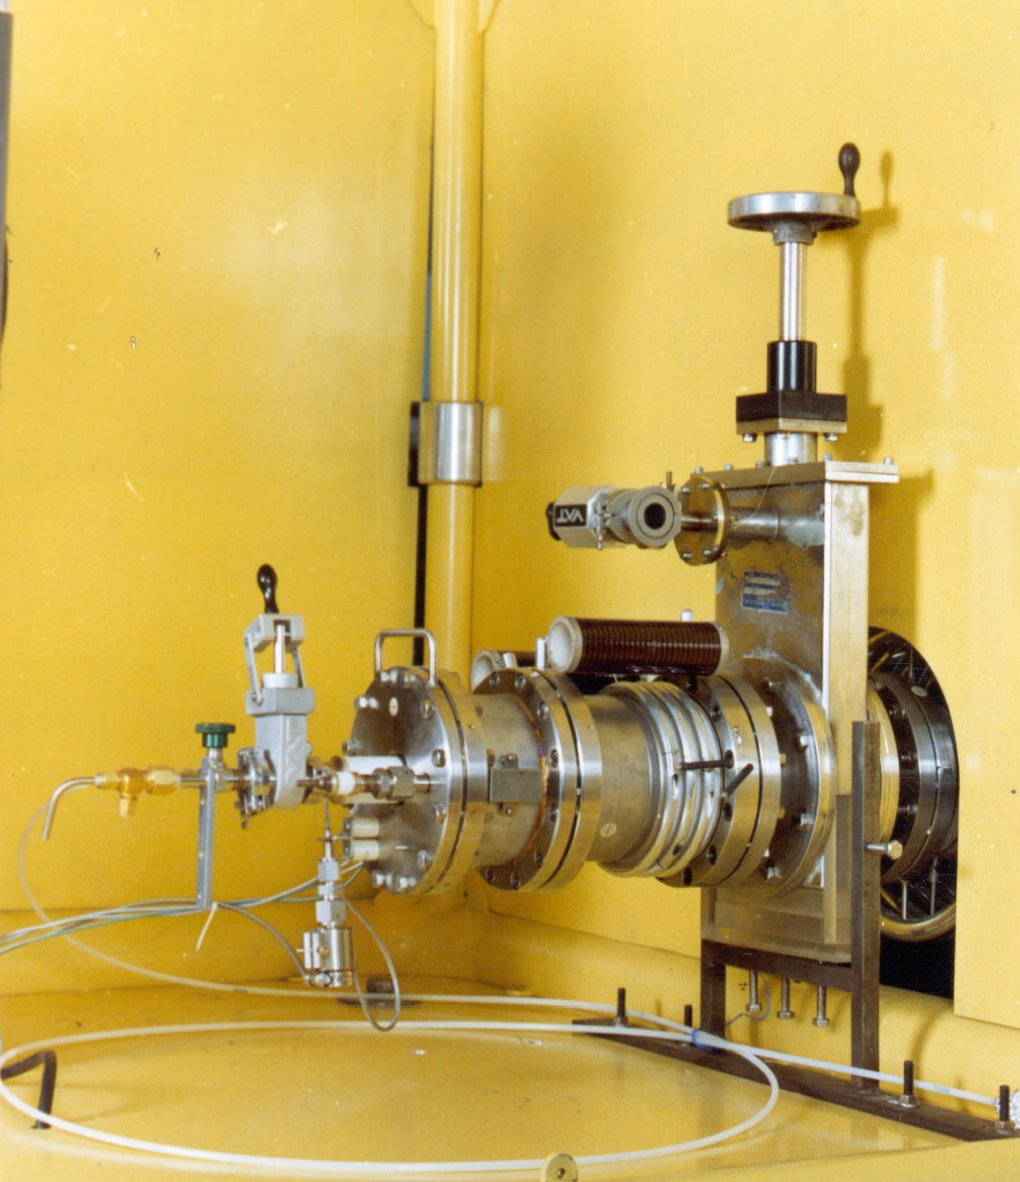
\includegraphics[scale=0.1]{SNICS.jpg}
   \end{center}
  
   
  \begin{itemize}
   
    \item FOTIA uses Source of Negative Ion by Caesium Sputtering \textbf{(SNICS)} as its ion source.
    \item \textbf{SNICS} generate negative ions by means of Caesium sputtering.
    \item Sample is put on the cathode stem.
    \item Positive extraction voltage is used to extract negative ion beams.
    \item Amount of beam current is dependent on the filament current and cathode voltage.
    \item Ion source must be kept under $10^{-7}$ mbar order of vacuum to protect Caesium.
   
   \end{itemize}

\end{frame}


\begin{frame}{FOTIA Subsystems-Bending \& Focusing Devices:Electrostatic Devices}

  \begin{itemize}
   
   
    \item Beam can be focused and bend with electrostatic devices.
    \item Accelerating section pre accelerate the beam after ion source.%High voltage power supply is used to setup pre acceleration voltage.
    \item FOTIA has electrostatic deflector which deflects the beam by $20^0$ in its path .
    \item FOTIA has a electrostatic quadrupole triplet to focus the beam.
    \item Accelerating tubes accelerate and focuses the beam.
    
   \end{itemize}

\end{frame}


\begin{frame}{FOTIA Subsystems-Bending and Focusing devices : Dipole Magnets}

  \begin{itemize}
   
    \item Two types of magnets are used in FOTIA. They are dipole and quadrupole magnets.
    \item Dipole magnets are used to bend the ion beam. There are four dipole magnets in FOTIA.
    \item First dipole magnet is just after ion source. It bends ion beam $70^0$ in its path. This magnet also acts as \textbf{mass selector} or \textbf{mass filter}.
    \item Second dipole magnet is at the terminal. This gives a bend of $180^0$. This magnet acts as \textbf{charge selector}.
    \item Third dipole magnet is after the accelerating tube. It bens beam by $90^0$. This also acts as \textbf{energy selector}.
    \item Fourth dipole magnet is at the experimental hall. This bends the beam to one of our three beam lines.
   
   \end{itemize}

\end{frame}

\begin{frame}{FOTIA Subsystems-Bending and Focusing devices:Quadrupole Magnets}

  \begin{itemize}
 
    \item Quadrupole magnets are used to focus the ion beam. In general quadrupole magnets are used as triplet to focus the beam on both plane.
    \item There are four quadrupole magnets in each beam line of FOTIA.  
    \item Quadrupole magnets are essential to deliver right size of the beam at the target. 
      
   \end{itemize}

\end{frame}



\begin{frame}{FOTIA Subsystems-High Voltage and High Current Power Supplies}

  \begin{itemize}
      
    \item Stability of the beam is a primary requirement of experimenters.
    \item To maintain stability of the beam highly stable power supplies are used to create magnetic field in magnets and electric field in electrostatic equipments. 
    \item All power supplies of the FOTIA have stability 100 ppm or better.
           
   \end{itemize}

\end{frame}


\begin{frame}{FOTIA Subsystems-Ultra High Vacuum System}

  \begin{itemize}
      
    \item Throughout the length of beam line vacuum of the order of $10^{-8}$ mbar is maintained. This is a mandatory requirement for proper running of any particle accelerator.
    \item Distributed vacuum pumping system is employed to avoid vacuum gradient. 
    \item FOTIA uses Turbo Molecular Pump backed by oil sealed rotary pump , diffusion pump and sputter ion pump for vacuum pumping.
    \item Pirani and cold cathode combination "Full Range" vacuum gauges are used for vacuum measurement at various location.
           
   \end{itemize}

\end{frame}

\begin{frame}{FOTIA Subsystems-High Voltage System}

  \begin{figure}
        \centering
        \begin{subfigure}[b]{0.5\textwidth}
                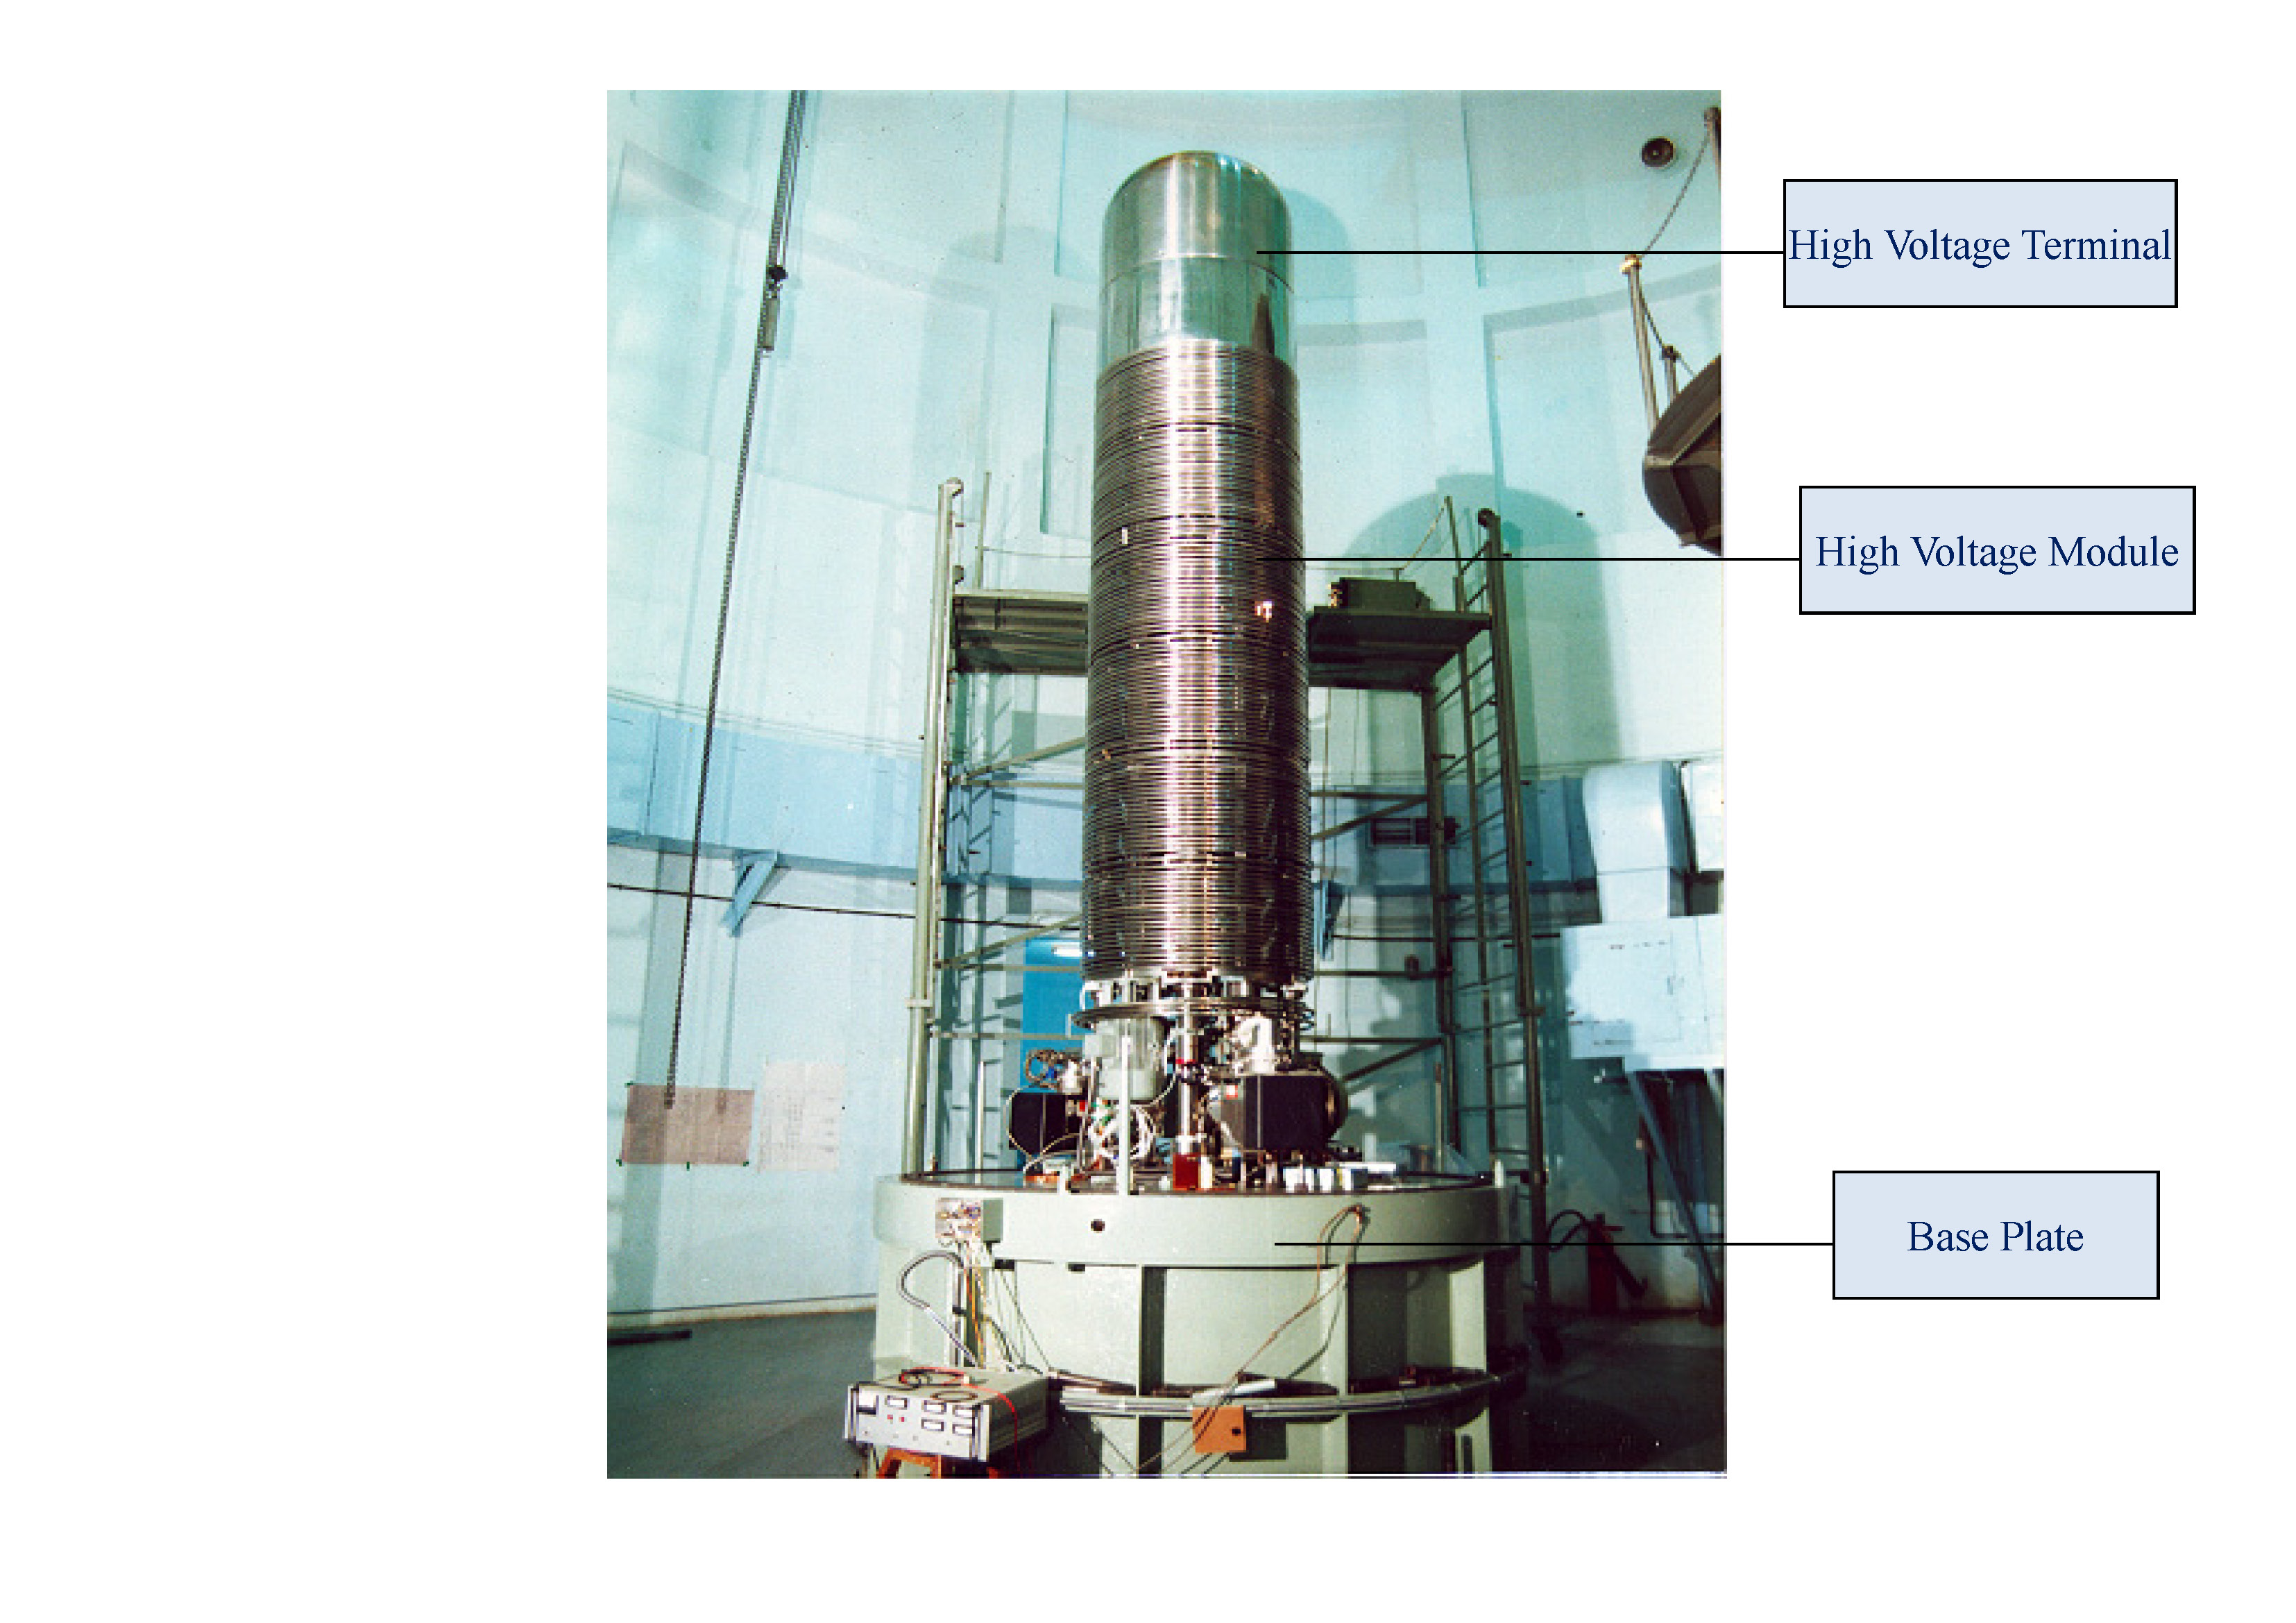
\includegraphics[width=\textwidth]{FOTIA_Page_08.jpg}
                \caption{FOTIA Column}
                \label{fig:FOTIA Column}
        \end{subfigure}%
        ~ %add desired spacing between images, e. g. ~, \quad, \qquad, \hfill etc.
          %(or a blank line to force the subfigure onto a new line)
        \begin{subfigure}[b]{0.5\textwidth}
                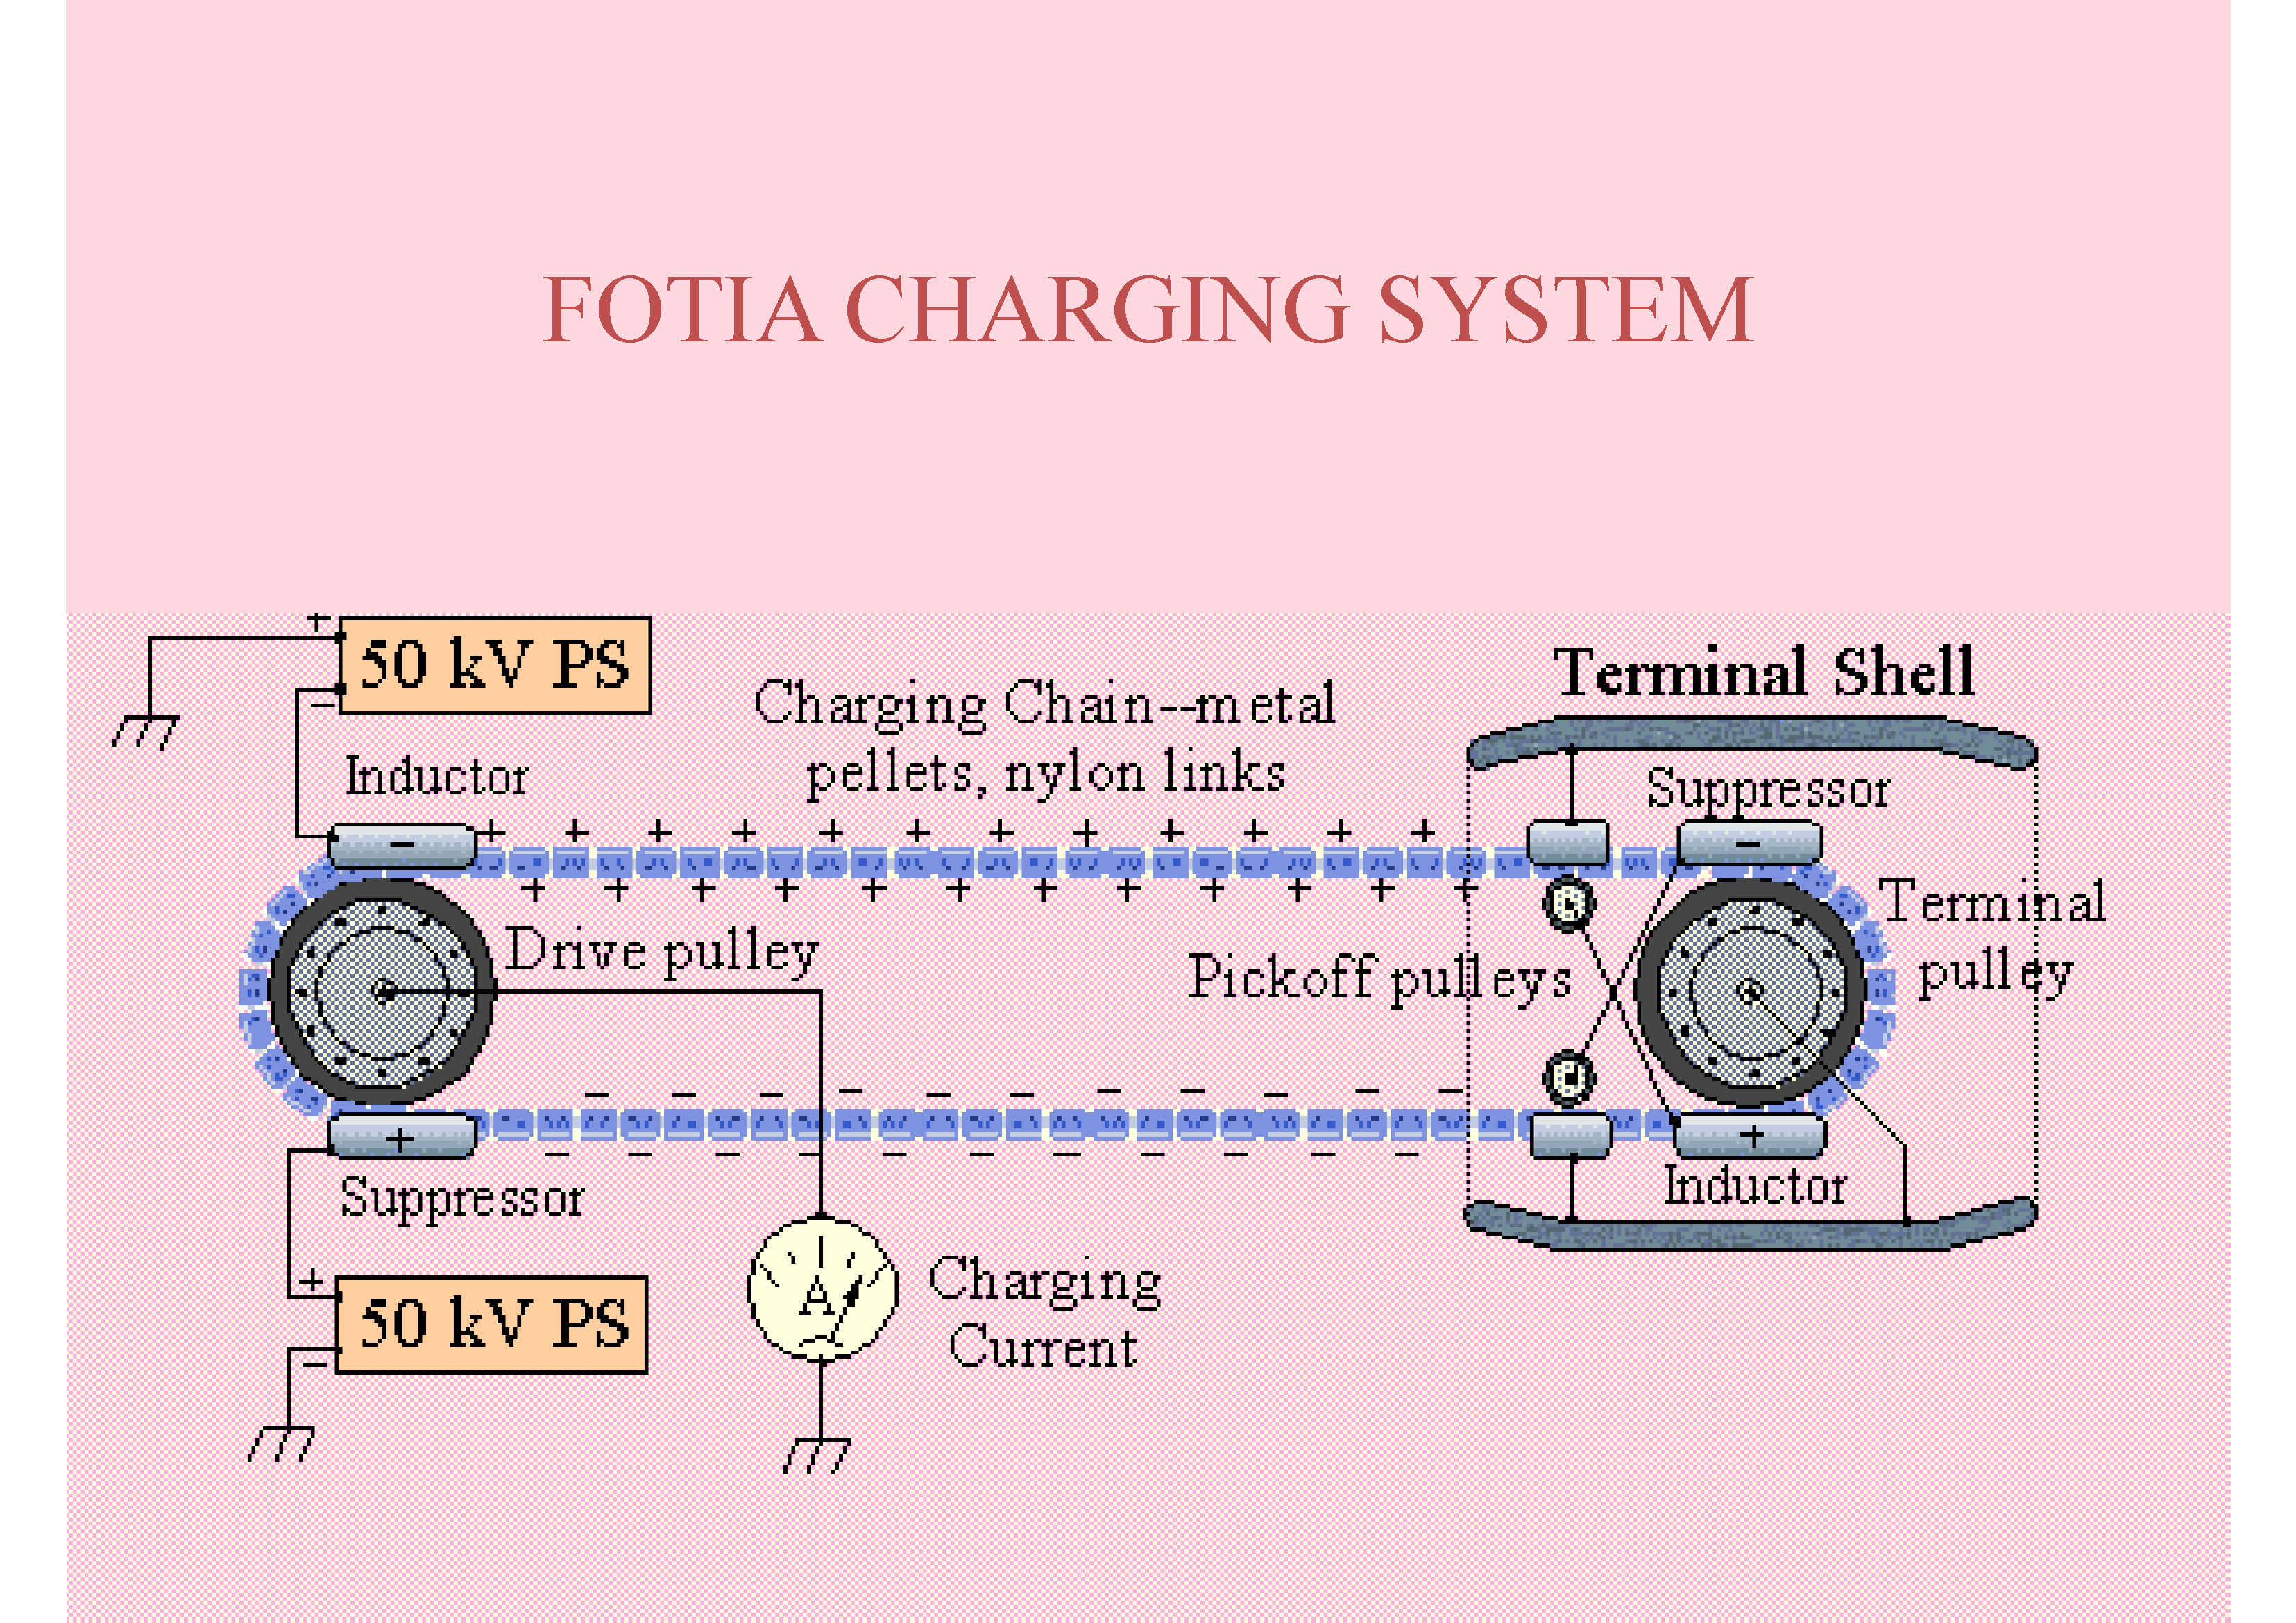
\includegraphics[width=\textwidth]{FOTIA_Page_10.jpg}
                \caption{Pellete Charging System}
                \label{fig:Charging System}
        \end{subfigure}
       
        \caption{Components of high voltage system}\label{fig:high voltage system}
\end{figure}
  
  
  
  \begin{itemize}
      
    \item Energy of beam is dependent on high voltage of terminal.
    \item Pellet charging system is used for generating very high voltage. 
       
   \end{itemize}





\end{frame}



\begin{frame}{FOTIA Subsystems-High Voltage System (cont)}

   \begin{itemize}
    \item Voltage gradient is maintained by allowing leakage current to pass through very high value ( 3 G$ \Omega$) resistance chain.
    \item Equipotential rings are used to maintain uniform electric field.
    \end{itemize}

\begin{figure}
        \centering
        \begin{subfigure}[b]{0.5\textwidth}
                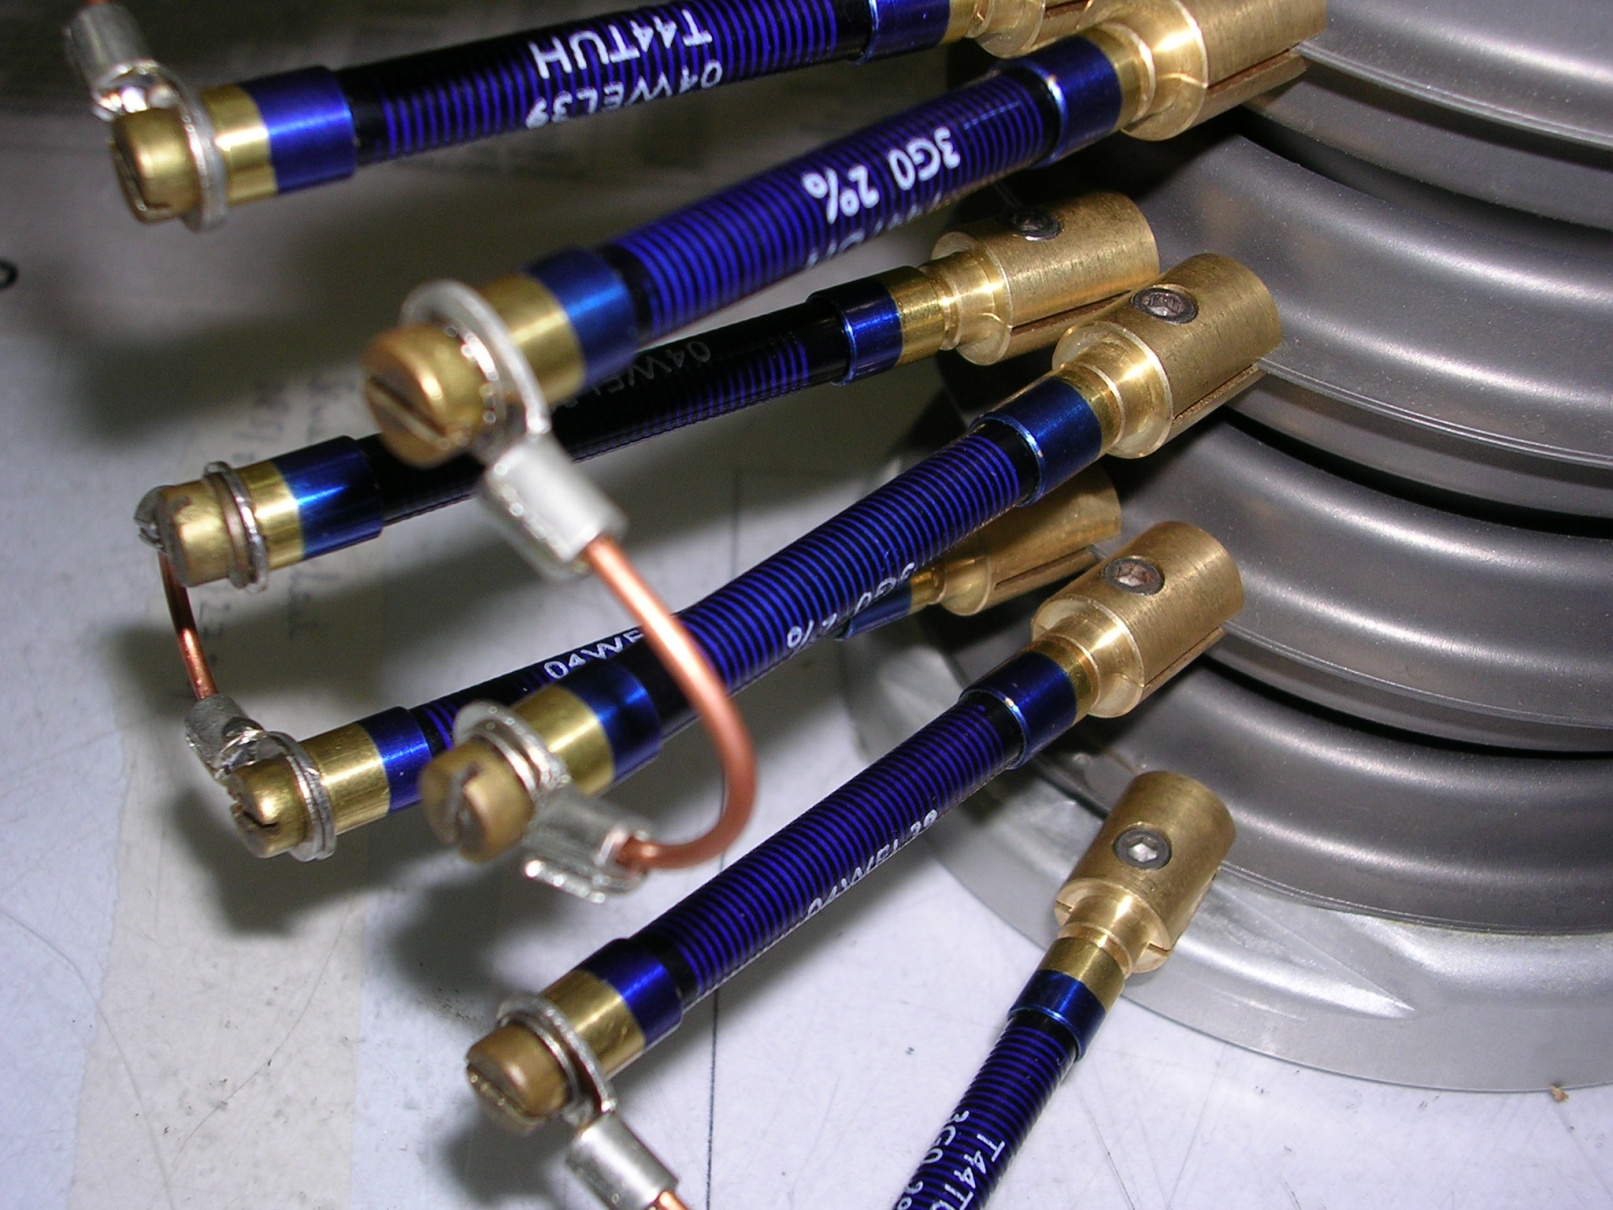
\includegraphics[width=\textwidth]{Resistor_chain.jpg}
                \caption{Resistor Chain}
                \label{fig:Resistor Chain}
        \end{subfigure}%
              
        \caption{Component of high voltage system}\label{fig:Component of High voltage system}
\end{figure}





\end{frame}

\begin{frame}{FOTIA Subsystems-$SF_{6}$ gas handling system}

  \begin{itemize}
      
    \item High purity $SF_{6}$ gas at 90 psig pressure is used for providing very high dielectric strength to hold the terminal voltage.
    \item $SF_{6}$ gas is recirculated to remove breakdown products, moisture and heat. 
    \item A separate storage tank is used to store the gas in case of tank opening.            
   \end{itemize}

\end{frame}



\begin{frame}{FOTIA Subsystem-Control System}

  \begin{itemize}
      
    \item FOTIA control system is a network based control system.
    \item It has two tier client server architecture.
    \item Computer Automated Measurement And Control(CAMAC) acts as as server.
    \item Operator workstation acts as client. Operator GUI is written in Qt 3 in Linux OS ( Fedora 7).
    \item Control system deals with 128 analog inputs , 64 analog outputs , 128 digital inputs and 96 digital outputs.
    \item Fibre optic link is used to transmit signal to the devices floating at high voltage.
      
           
   \end{itemize}

\end{frame}


\begin{frame}{FOTIA Subsystem-Measurement and Instrumentation}

  \begin{itemize}
      
    \item Faraday Cup is used to measure the beam current.
    \item Beam Profile Monitor(BPM) provide shape and size of the beam.
    \item Generating Volt Meter (GVM) is used to measure high voltage of the terminal.
    \item Hall probe is used to measure the magnetic field. Current readback of current power supply is also used to measure magnetic field.         
   \end{itemize}

\end{frame}




\begin{frame}{FOTIA Beam Lines}

FOTIA has five dedicated beam lines to perform five different types of experiments. They are  
  \begin{itemize}
      
    \item Nuclear physics experiments.
	\item Proton Induced Positron Annihilation Spectroscopy (PIPAS) experiments.
	\item Trace Element Analysis ( RBS, PIXE, etc.) experiments.
	\item Irradiation line for Material science experiments.
	\item Radiation biology experiments.
            
   \end{itemize}

\end{frame}

\begin{frame}{Nuclear Physics and Irradiation experiments}

  \begin{figure}
        \centering
        \begin{subfigure}[b]{0.5\textwidth}
                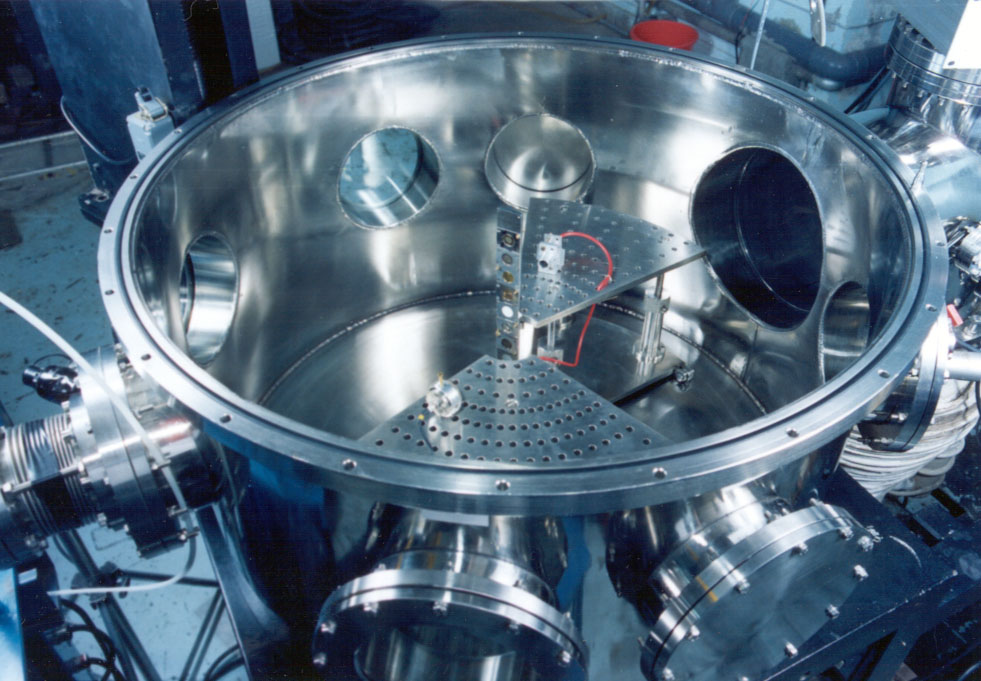
\includegraphics[width=\textwidth]{Scattering_chamber.jpg}
               % \caption{External PIXE Setup-1}
               % \label{fig:External PIXE Setup-1}
        \end{subfigure}%
               
        \caption{General Purpose Scattering Chamber}\label{fig:Scattering Chamber}
\end{figure}
  
  
  \begin{itemize}
    
    \item Nuclear Physics and general irradiation experiments are carried out in general purpose scattering chamber . 
			           
   \end{itemize}


\end{frame}


\begin{frame}{Proton Induced X ray Emission (PIXE)}

  \begin{figure}
        \centering
        \begin{subfigure}[b]{0.3\textwidth}
                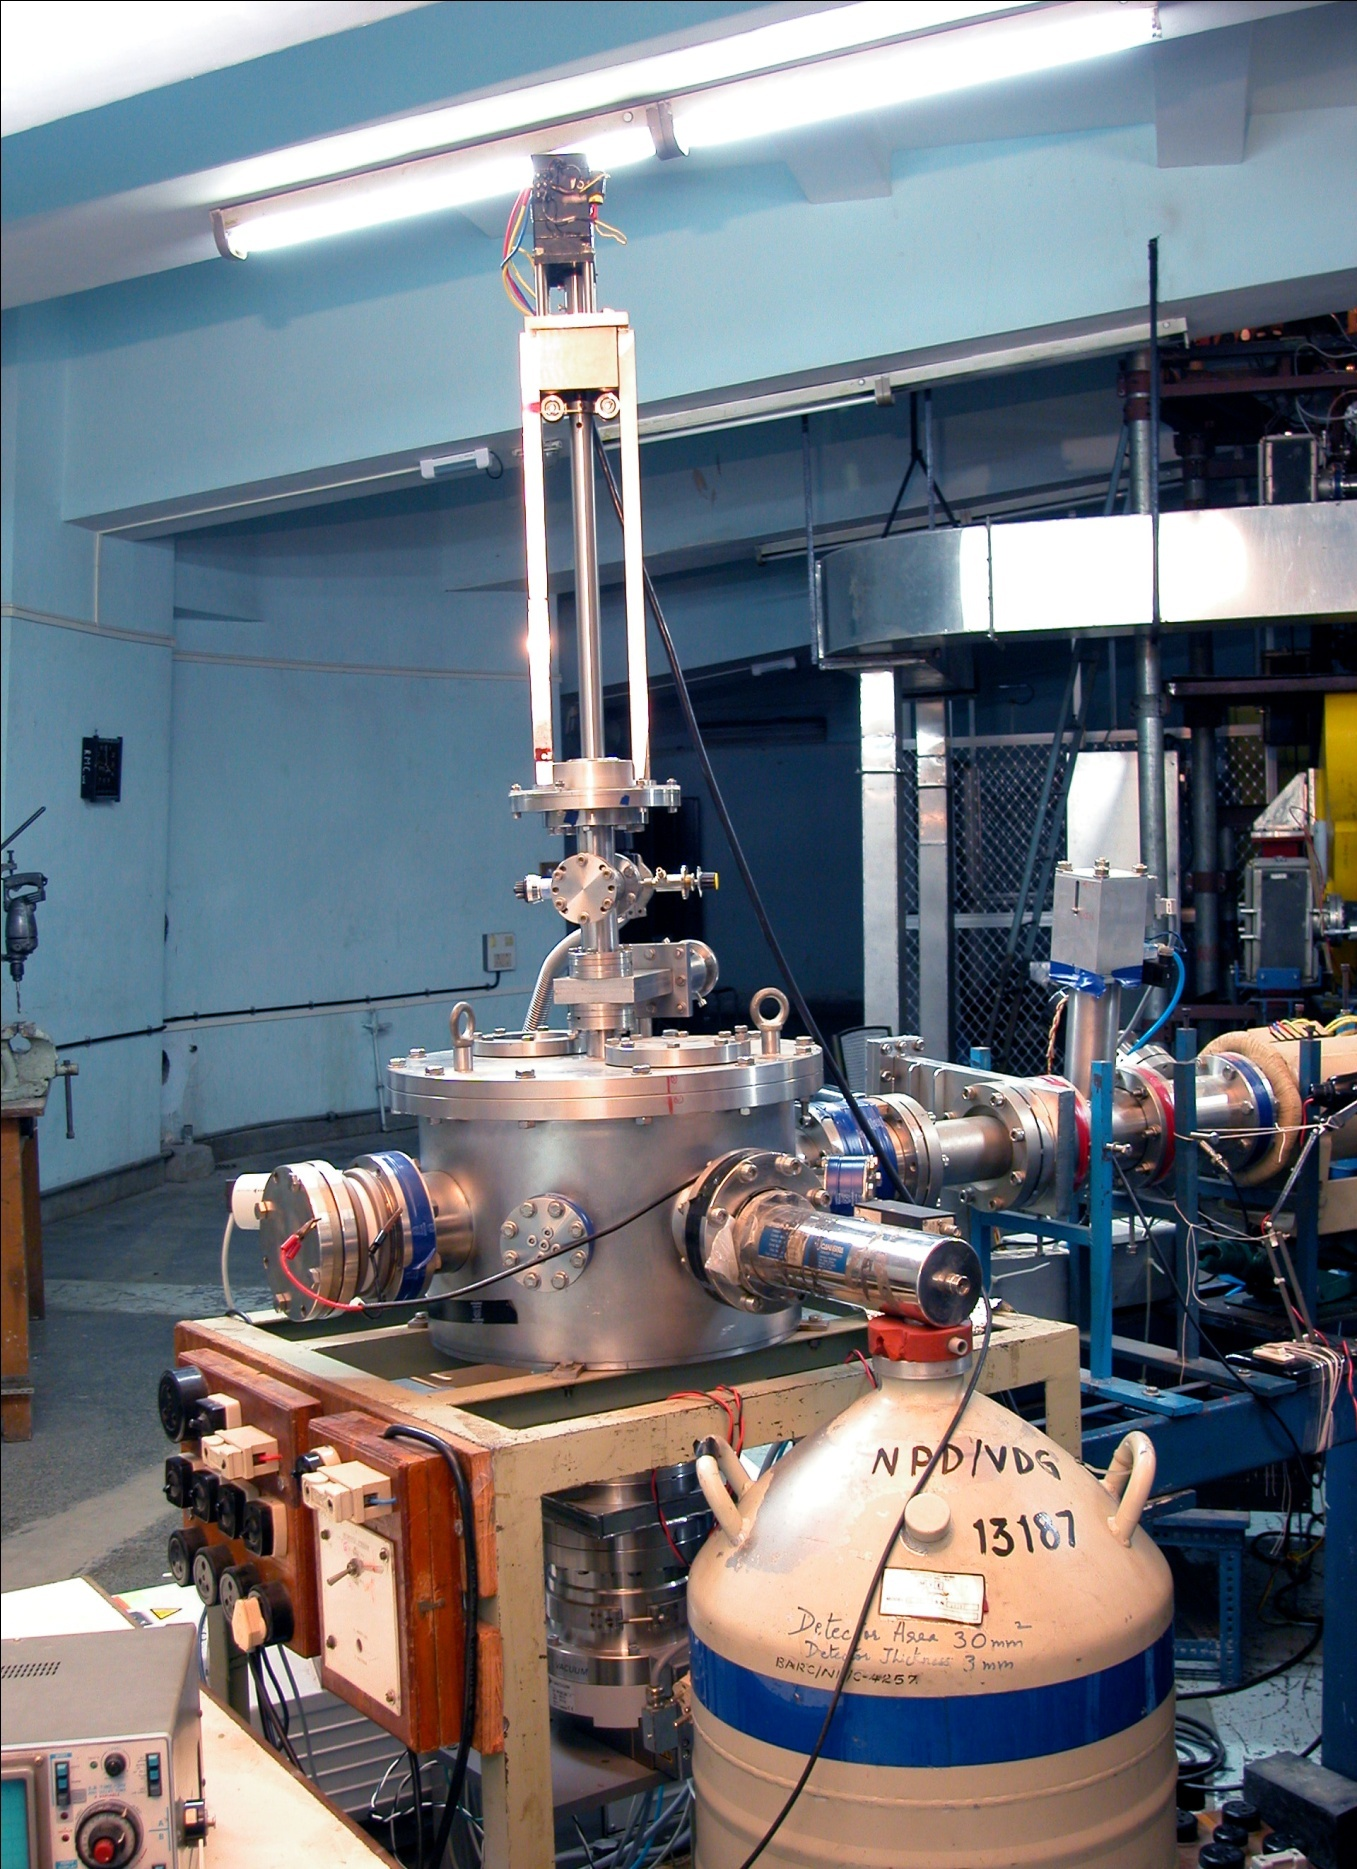
\includegraphics[width=\textwidth]{Pixe_setup.jpg}
               % \caption{External PIXE Setup-1}
               % \label{fig:External PIXE Setup-1}
        \end{subfigure}%
               
        \caption{PIXE Setup}\label{fig:PIXE Setup}
\end{figure}
  
  
  \begin{itemize}
    
    \item Proton beam, when fall on the target material ,material  emit different energy x rays according to its composition. 
	\item Detecting X rays, composition of the material can be determined very accurately.
		           
   \end{itemize}


\end{frame}






\begin{frame}{External PIXE \& Radiation Biology}

  \begin{figure}
        \centering
        \begin{subfigure}[b]{0.3\textwidth}
                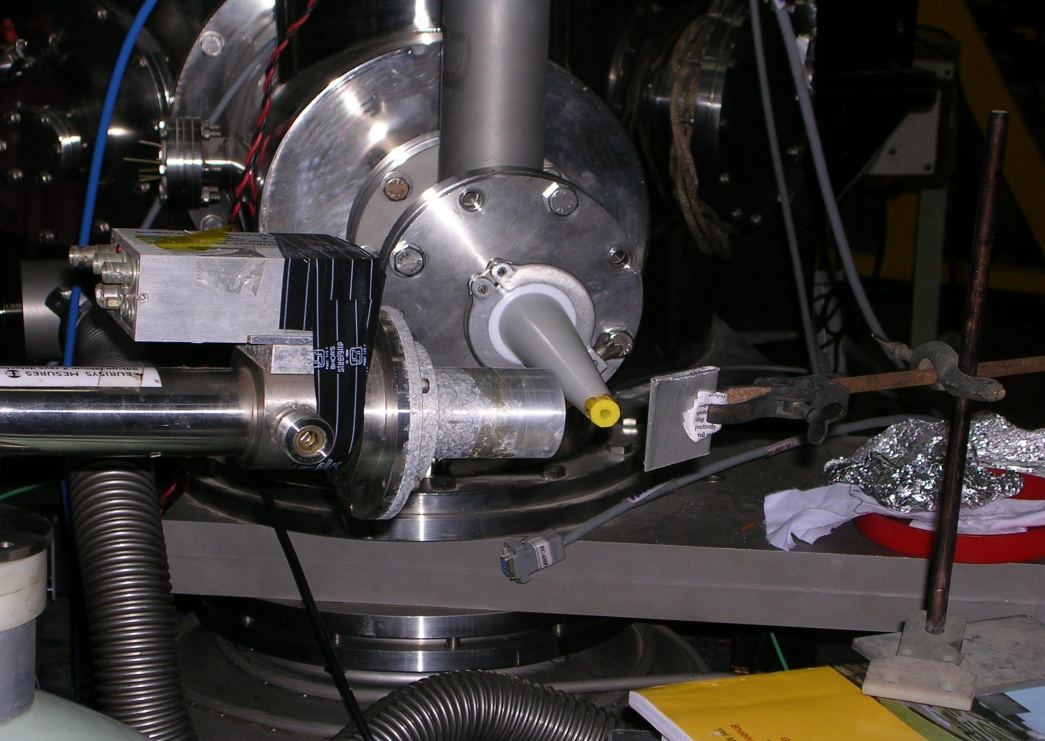
\includegraphics[width=\textwidth]{External_pixe1.jpg}
               % \caption{External PIXE Setup-1}
               % \label{fig:External PIXE Setup-1}
        \end{subfigure}%
        ~ %add desired spacing between images, e. g. ~, \quad, \qquad, \hfill etc.
          %(or a blank line to force the subfigure onto a new line)
        \begin{subfigure}[b]{0.3\textwidth}
                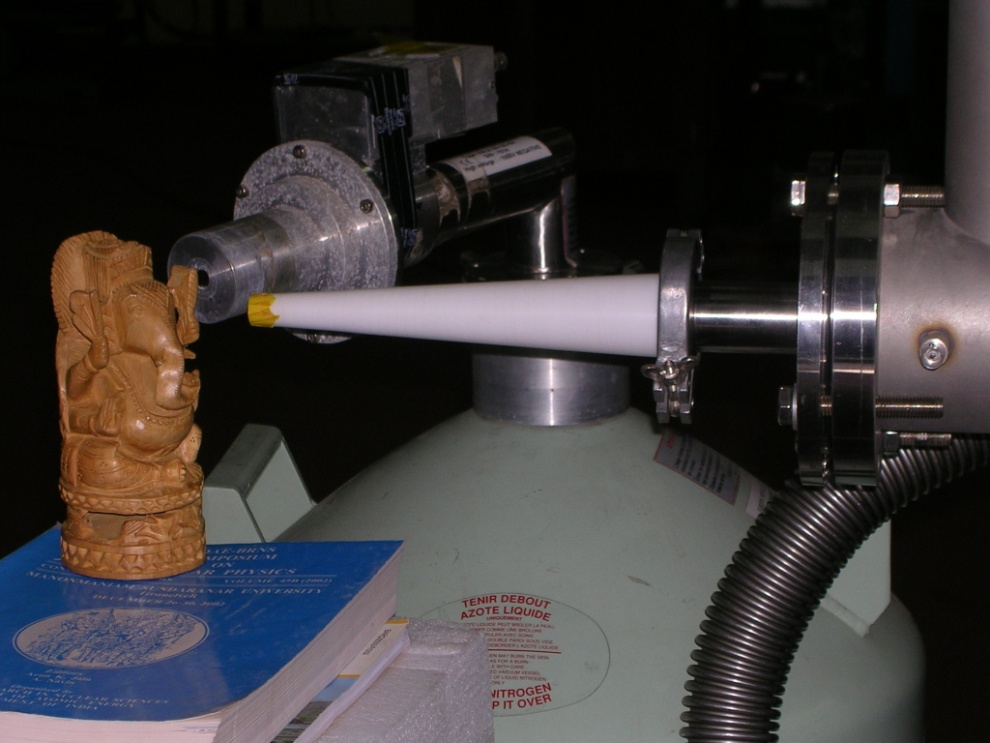
\includegraphics[width=\textwidth]{External_pixe2.jpg}
               % \caption{External PIXE Setup-2}
               % \label{fig:External PIXE Setup-2}
        \end{subfigure}
       
        \caption{External PIXE Setup}\label{fig:External PIXE Setup}
\end{figure}
  
  
  \begin{itemize}
     
    
    \item A thin (Ti 20 $\mu m$) or (Kapton 8 $\mu m$) window is placed at the end of beam line to take the beam. 
	\item Proton beam of varying intensities are taken out in air.
	\item Radiation biology, Environment assessment and Evaluation of documents and other material for forensic application  programme use beam in air.
	           
   \end{itemize}


\end{frame}


\begin{frame}{Some notable experiments}
  
  
  \begin{itemize}
     
    
    \item Simulation of neutron damage of stainless steel in reactor by proton beam. 
	\item Photon Induced Positron Annihilation Spectroscopy (PIPAS).
	\item PIXE studies of Gall bladder stones .
	\item Determination of material composition for Archaeological sample.
	\item Quadrupole testing for the project X of Fermi lab , USA.          
    \item Characterisation and calibration of various equipements to be used in upcoming Low Energy High Intensity Proton Accelerator(LEHIPA).
    \item Nuclear detector calibration.
   \end{itemize}


\end{frame}

\begin{frame}{FOTIA Operational Statistics}
  
  
  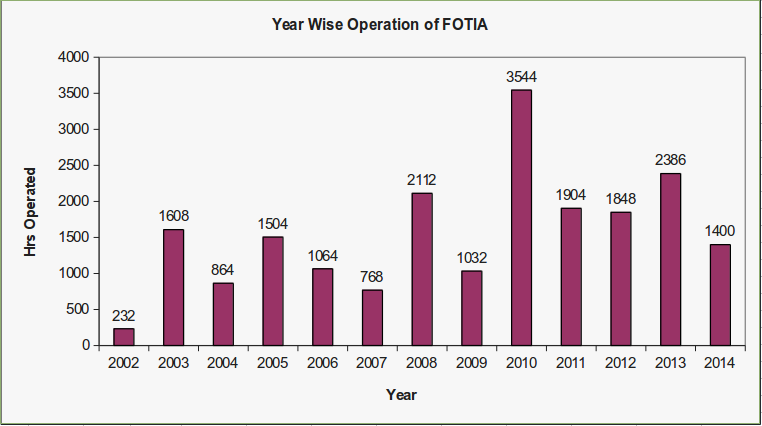
\includegraphics[width=\linewidth]{operational_data.png}


\end{frame}

\begin{frame}{Safety aspects in FOTIA}

  \begin{figure}
        \centering
        \begin{subfigure}[b]{0.6\textwidth}
                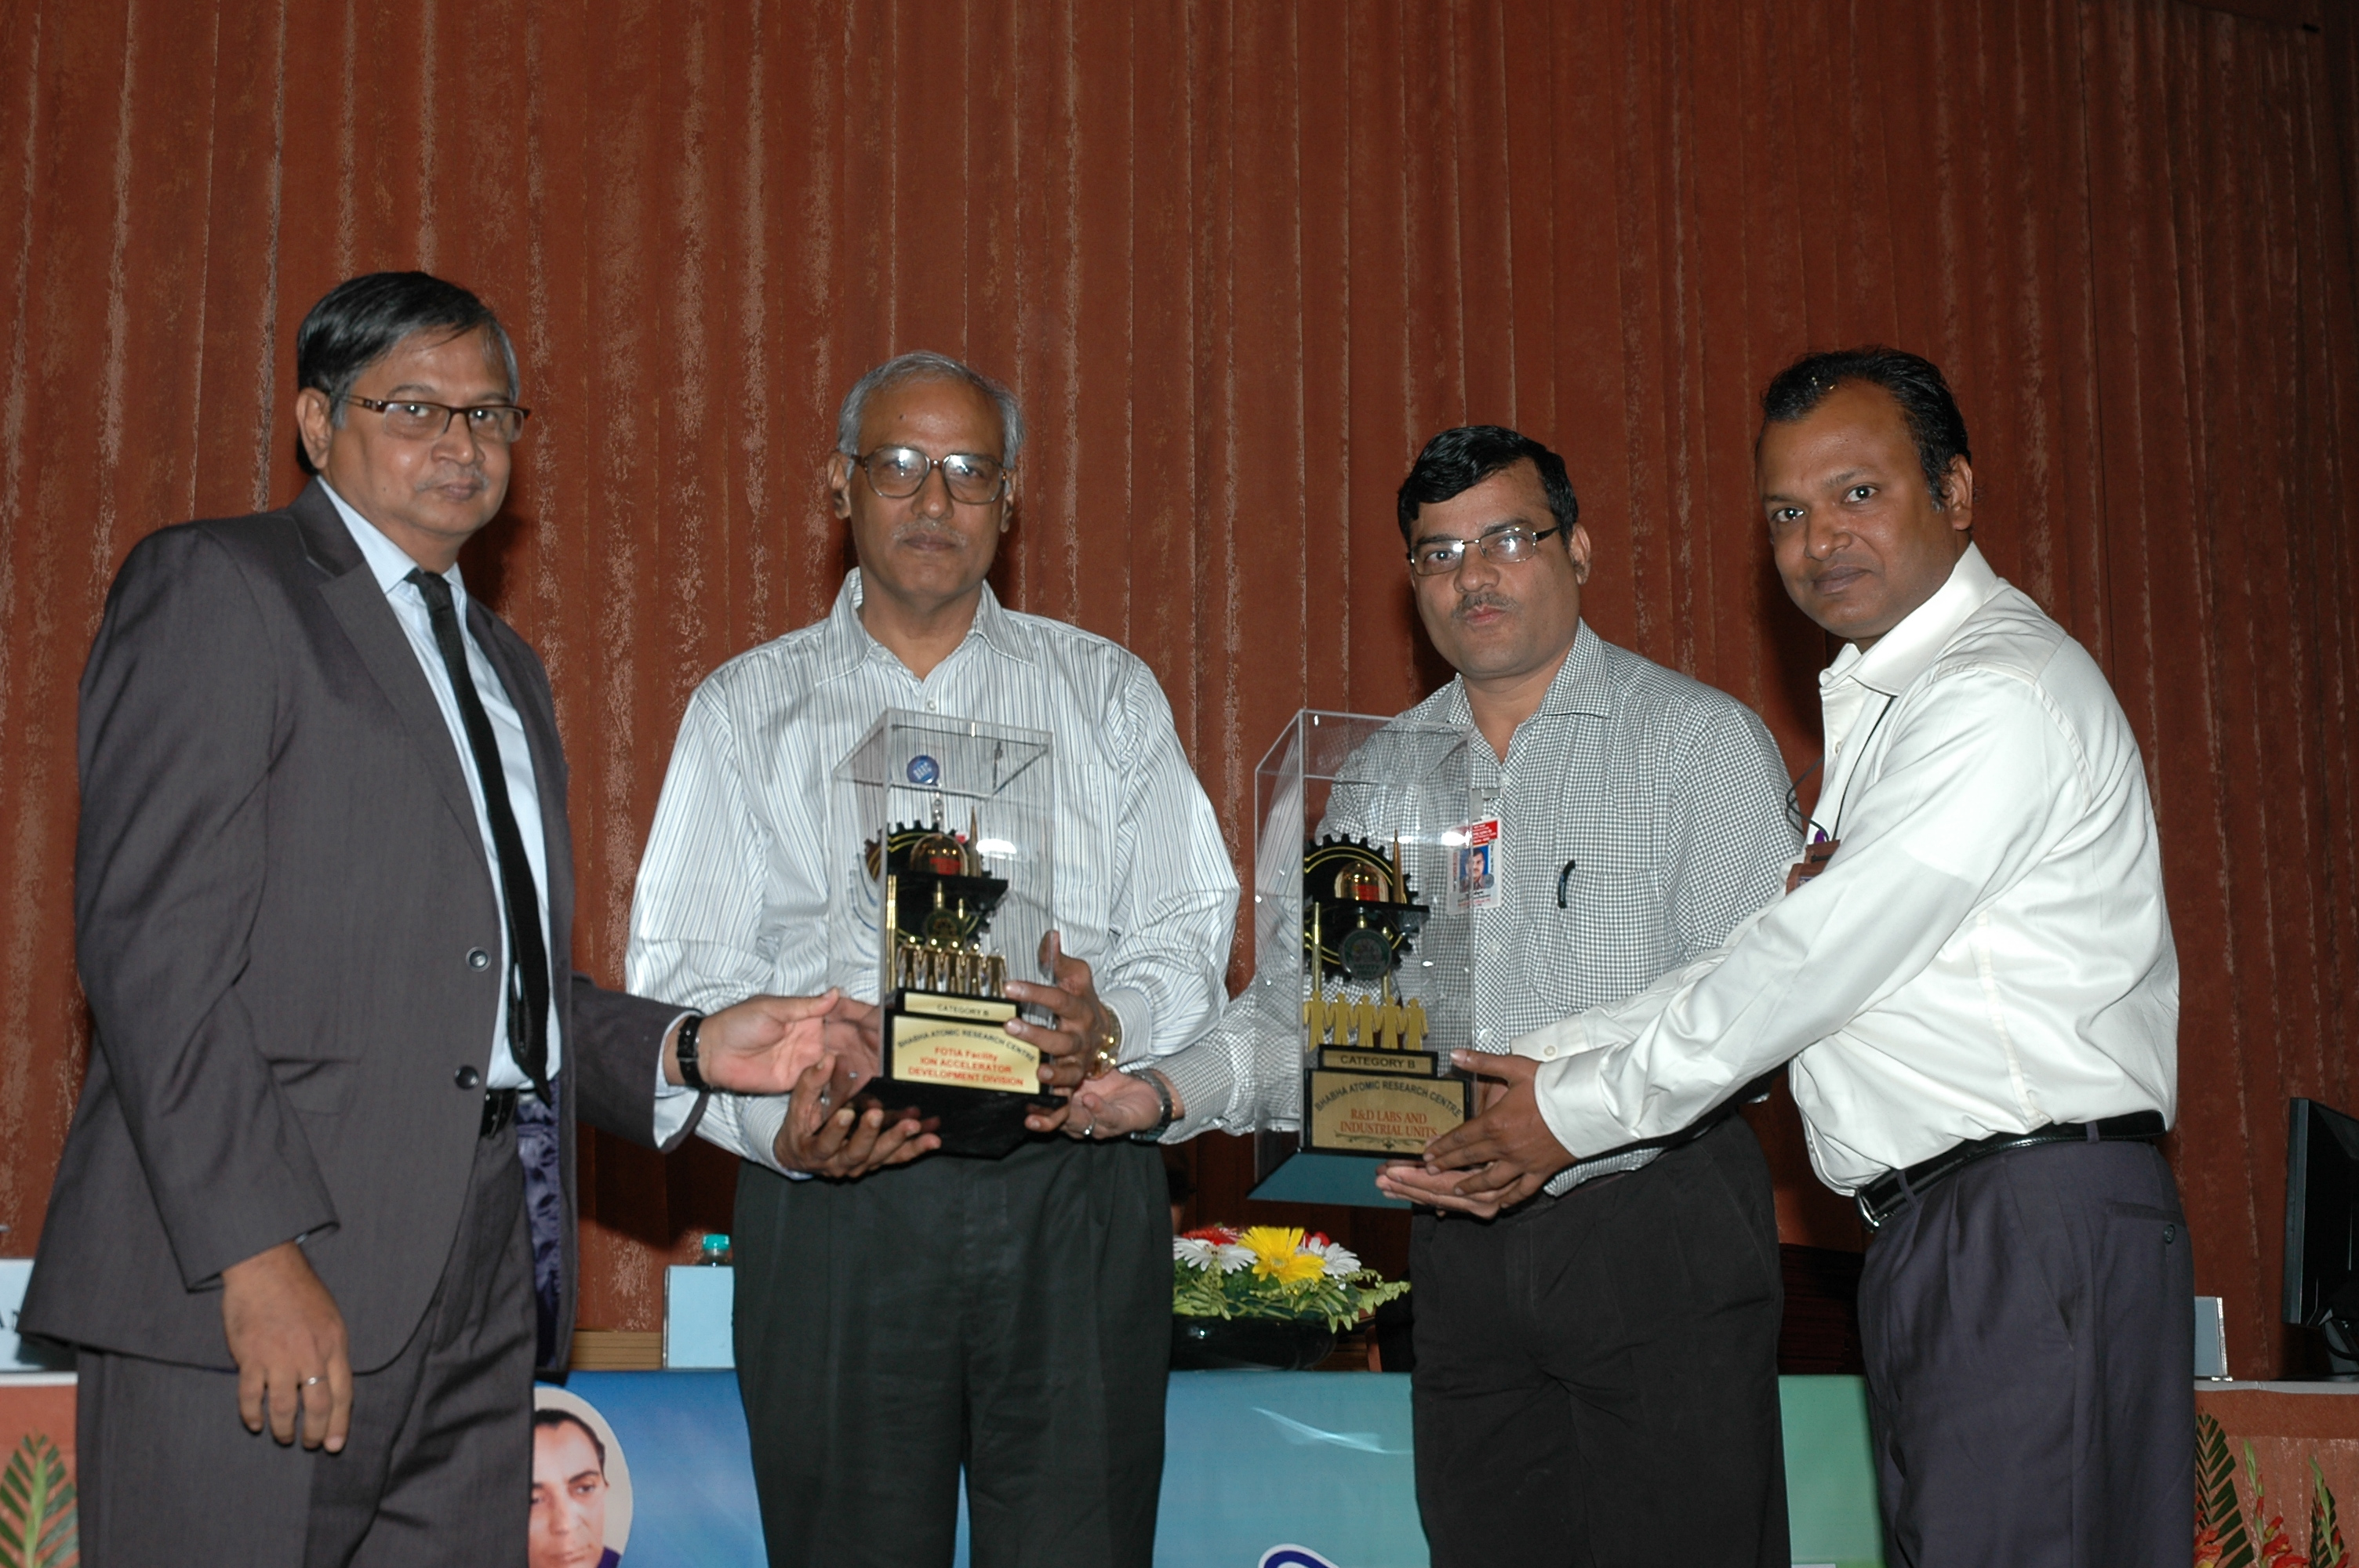
\includegraphics[width=\textwidth]{DSC_0067.jpg}
                %\caption{FOTIA Column}
                %\label{fig:FOTIA Column}
        \end{subfigure}%
               
        \caption{Wining Safety Shield}\label{fig:Wining Safety Shield}
\end{figure}
  
   
  
  \begin{itemize}  
    \item FOTIA is one of the safest accelerator in operation. It won safety shield for three consecutive years(2011 to 2013).
    \item FOTIA is regulated by Unit Level Safety Committee-Particle Accelerator (ULSC-PA). Many of FOTIA practices are recommended to other accelerator facilities by ULSC-PA.           
   \end{itemize}

\end{frame}

\begin{frame}{Safety in FOTIA}
Safety aspects of FOTIA can be classified as 
 \begin{itemize} 
 \item Human Safety.
 \item Equipment Safety.
\end{itemize} 
\end{frame}

\begin{frame}{Human Safety in FOTIA}
Human safety is of utmost importance because it can’t be compensated.\\
	
Human safety involves the safe working condition for 
 \begin{itemize} 
 \item Electrical Systems
 \item Mechanical Systems
 \item Radiation 
 \item General Industrial Safety.
\end{itemize}		
To ensure human safety three strategies are followed. 
\begin{itemize}
\item Training of the personnel.
\item Audio Visual alarm and deterrent notices such as "No Entry" etc .
\item Different guiding notices such as "Exit" , "Emergency Exit" , "Fire Exit" , "Assembly point" etc
\item Emergency response procedure ( such as "Actions to be taken in case of electric shock") posters.  
\item Automatic interlock protection in case of human mistakes. 
\end{itemize}	 
 
\end{frame}

\begin{frame}{Human Safety in Electrical System}

 \begin{itemize} 
 \item All the high voltage areas are properly marked and DANGER notice is put up to prevent a person to approach nearby.
\item High voltage area of  deck power supply is enclosed by the protective cage and cage door is interlocked with the high voltage power supply in such a way that if, the cage door is open then power supply can’t be switched ON.
\item If the power supply is ON and cage door is opened, then immediately power supply will automatically get switched off.
\item An earthing rod is provided to discharge the deck, after entry, the cage should be grounded, which ensures that if by mistake power supply remained ON, still it will be at ground potential, thereby ensuring safety of working personnel. 
\item All the electrical equipments are ISI certified.
 \item High voltage and high current cables are marked and laid properly as per Indian Electricity rule.
\item Earthing resistances are ensured to be below allowed values and checked regularly. 
\end{itemize}		
	 
 
\end{frame}


\begin{frame}{Human Safety- Mechanical System}

 \begin{itemize} 
 \item Personnel are required to wear helmet and safety shoes when they are working in the accelerator room.
 \item All high pressure area are marked with DANGER notice. Pressure value of accelerator and storage tank are always monitored.
 \item Pressure  Release Safety valve of compressors are set at 10\% above the working pressure and well below the design limit.
 \item Heavy objects, such as gas cylinders etc. are tied securely with the chain. 
\end{itemize}		
	 
\end{frame}



\begin{frame}{Human Safety- Radiation}
Though radiation level in FOTIA is minimal but no lapses are allowed dealing with radiation related issues.
\begin{itemize} 
 \item All the radiation area are marked and DANGER notices are  displayed.
 \item Gamma monitors and Neutron detectors continous monitor the radiation level.An audio visual alarm is automatically generated if radiation detectors pick up radiation above the permissible limit.
 \item During accelerator operation, the radiation level is monitored periodically by health physicist. 
 \item Personnel must wear the TLD and fast neutron badges.
 
 \item FOTIA employs search and secure interlock system to ensure that no person can be trapped in the accelerator room or beam hall during accelerator operation and receive high radiation dose. 
\end{itemize}		
	 
 
\end{frame}


\begin{frame}{General Industrial Human Safety}

\begin{enumerate} 
 \item \textbf{Fire and Chemical safety:}
  Adequate  smoke detectors are installed  throughout the building. In case of smoke or fire audio alarm is generated and visual indication is available at fire alarm pane to identify the troubled zone
 \item \textbf{Safety against Inflammable material:}
 During sample change or Caesium loading, inert atmosphere of Argon gas is maintained and personnel are required to wear the proper safety gadgets while handling Caesium.
 \item \textbf{$SF_6$ leakage:}
 $SF_6$ monitors and Oxygen deficiency monitors are provided. In case of $SF_6$  leak audio / visual alarm is generated and if oxygen level falls below 19.0 \%,  building  will be evacuated.
\item \textbf{General industrial safety:}
Protective helmets, Protective gloves, safety belts and safety shoes are available for use if required.
\end{enumerate}		
	 
 
\end{frame}


\begin{frame}{Equipment Safety}
Safety Interlocks are provided to ensure automatic operation during fault condition in fail safe mode. Two levels of interlocking arrangement have been provided 
\begin{enumerate} 
 \item \textbf{PLC based:}
  \begin{itemize}
  \item  Charging chain  motor, Rotating shaft motor
  \item  $SF_6$  Compressor, Blower, Rotary pump
  \item  $SF_6$  Monitors, Oxygen deficiency Monitors, Radiation Monitors
  \item  Rouging pumps, Ion pumps, Isolation valves 
  \end{itemize} 
 \item \textbf{Hard-wired:}
\begin{itemize}
\item  Cage door with the pre-acceleration voltage.
\item  Cathode cooling pump with isolation transformer.
\item  GVM with TRV
\item  Turbo pump valve with Ion Gauge Controller.
\item  Fast acting valve with Ion Gauge Controller-1 \& Ion Gauge Controller-2.
\end{itemize} 
\end{enumerate}		
	 
 
\end{frame}

\begin{frame}{Safety motto of FOTIA}
FOTIA team believe in following two dictum
\begin{itemize}
\item Know safety, no injury.\\
     No safety, know injury. \\
      -- Author Unknown			
\item \textbf{Safety is a mission not an intermission.} 
\end{itemize} 

FOTIA staffs know safety. As a result FOTIA till today has never faced pain of any injury or equipment damage.\\
Since safety is a mission 
\begin{itemize}
\item 	All the sensors, safety equipments, interlock systems are periodically tested and maintained.
\item 	We are always open to the suggestions which can improve our facility's safety.	
 
\end{itemize} 

\end{frame}



\begin{frame}{Conclusions}
\begin{itemize}

\item \textbf{FOTIA} is running very reliably for last ten years and contributed to various program of DAE.

\item \textbf{FOTIA} follows stringent safety norms to ensure human and equipment safety.

\item \textbf{FOTIA} design, installation and operational experience are being utilized to design and commission next generation bigger and more complex accelerators.

\item \textbf{FOTIA} has a smaller cousin known as Low Energy Accelerator Facility ( LEAF) . This is a Low energy ( upto 50 keV ) high current( order of hundreds of nano ampere) negative ion accelerator. This accelerator is also running very successfully and produced very high quality international papers. Three PhD students of IIT Bombay have extensively used this facility for their research work.



\end{itemize}
\end{frame}

\begin{frame}{Conclusions}
 \textbf{The FOTIA team invite all possible users from BARC and outside research community to make use of both the facilities which is delivering variety of ion beams for research within BARC premises.}\\
 
 \begin{center}
  \huge {Thank You.}
\end{center}
\end{frame}
\end{document}

===============================================

